\textbf{Re-visiting the Computation Challenge}~~
\begin{figure}
  \vspace{-7pt}
    \subfigure[Iterative Evaluation]{\label{fig:itERR}
      \begin{minipage}[l]{0.46\columnwidth}
        \centering
        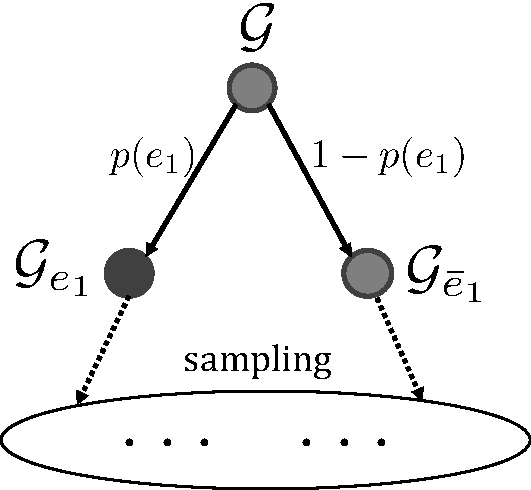
\includegraphics[height=2.7cm]{ill/iterativeERR.pdf}
      \end{minipage}
      }
    \subfigure[Memorized Evaluation]{\label{fig:groupERR}
      \begin{minipage}[l]{0.46\columnwidth}
        \centering
        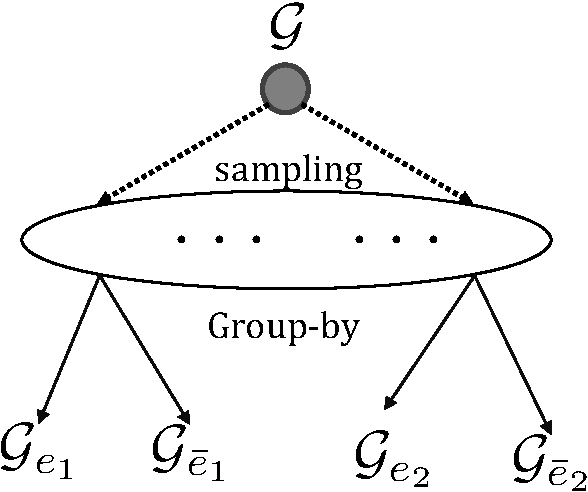
\includegraphics[height=2.7cm]{ill/groupERR.pdf}
      \end{minipage}
      }
    \vspace{-5pt}
    \caption{Sampling-based reliability detection}
    \label{fig:computationERR}
    \vspace{-7pt}
\end{figure} 
As ever mentioned, 
the evaluation of $\mathcal{E}RR(e)$ involves a fundamental problem concerning uncertain graphs, which we call 
the two-terminal reliability detection (TTR) problem. 
Since this problem is \#P-complete, we focus on efficiently and accurately approximate TTR.
The Monte-Carlo sampling method can be used to estimate the underlying reliability of an uncertain graph. 
Namely, we create a subset of possible worlds of the input uncertain graph with the use of edge sampling probabilities. 
Then, we take the average of the number of connected node pairs in the sampled worlds as an approximation. 
 
The $\mathcal{E}RR$ evaluation over all the edges is not trivial. 
One option is to iteratively invoke the sampling-based reliability computation over all the edges, 
as illustrated in Figure~\ref{fig:itERR}. 
It is straightforward to compute the connected components of a graph in linear time (regarding the numbers of the nodes and edges of the graph) using either breadth-first search or depth-first search.
For each edge, we need to perform the connected component detection for $N$ sampled graphs.
Thus, the overall time complexity is $\mathcal{O}(|E|\cdot N |E|)$.

Apparently, the baseline method is inefficient when the uncertain input graph is enormous.
XXXXX
Here, we present an efficient method which re-uses 
the connected components detection result of samples as illustrated in Figure~\ref{fig:groupERR}. 
For each edge $e$, we group the sampled possible worlds according to the edge existence, 
then get the average value of $cc$ over each group as accurate approximation of $cc(\mathcal{G}_{e})$ and $cc(\mathcal{G}_{\bar{e}})$.
The running time analysis roughly follows the analysis of the single-edge case.  
The overall time complexity is $\mathcal{O}(N |E|)$. 
By this way, we bring the evaluation of edge reliability relevance to the realm.